\documentclass{standalone}

\usepackage{fontspec}
\defaultfontfeatures{Ligatures=TeX}  % -- becomes en-dash etc.
\setmonofont{Fira Mono}[Scale=MatchLowercase]

\usepackage{tikz}
\usetikzlibrary{calc,patterns,quotes,tikzmark,angles,decorations.pathreplacing}
\tikzset{fontscale/.style = {font=\relsize{#1}}}
\usepackage{feynman-tikz}

% math
\usepackage{amsmath}
\usepackage{amssymb}
\usepackage{mathtools}
\usepackage{xfrac}


\usepackage[
  mathrm=sym,        % use math font for mathrm, not text font
  math-style=ISO,
  bold-style=ISO,
  sans-style=italic,
  nabla=upright,
  partial=upright,
  warnings-off={
    mathtools-colon,
    mathtools-overbracket,
  },
]{unicode-math}

\usepackage[
  separate-uncertainty=true,
  per-mode=symbol-or-fraction,
]{siunitx}
\sisetup{math-micro=\text{µ},text-micro=µ}


% new commands
\newcommand{\code}[2]{%
  \texttt{\textcolor{#1}{\detokenize{#2}}}%
}

\usepackage{xcolor}

% define your colors here
\xdefinecolor{bioblue}{HTML}{4c5b75}
\xdefinecolor{bredongreen}{HTML}{619645}
\xdefinecolor{honeywax}{HTML}{f9a825}
\xdefinecolor{protonred}{HTML}{a12b2b}
\xdefinecolor{electronblue}{HTML}{0099d1}
\xdefinecolor{gammagreen}{HTML}{0a9e74}

\xdefinecolor{tugreen}{RGB}{132, 184, 25}
\xdefinecolor{tulightgreen}{HTML}{99b560}
\xdefinecolor{darkmode}{HTML}{3a3d41}
\colorlet{tulight}{tugreen!20!white}
\colorlet{tudark}{tugreen!80!black}

\xdefinecolor{tuorange}{RGB}{227, 105, 19}
\xdefinecolor{tuyellow}{RGB}{242, 189, 0}
\xdefinecolor{tucitron}{RGB}{249, 219, 0}

\xdefinecolor{tublue}{RGB}{25, 132, 184}
\colorlet{tublight}{tublue!20!white}
\colorlet{tubdark}{tublue!60!black}

\xdefinecolor{yamlblue}{HTML}{a094f2}
\xdefinecolor{yamlgreen}{HTML}{00b300}
\xdefinecolor{yamlorange}{HTML}{d67c58}
\xdefinecolor{yamlpink}{HTML}{ff00ff}
\xdefinecolor{yamlyellow}{HTML}{ffd800}

\colorlet{lightgray}{darkgray!70!white}
\colorlet{lightergray}{darkgray!50!white}
\usepackage{pagecolor}

\setmainfont{Fira Sans}

% colours
\xdefinecolor{darkmode}{HTML}{3a3d41}
\xdefinecolor{cherenkov_blue}{HTML}{4066a3}

\tikzfading[name=fade30,
  left color=transparent!0, right color=transparent!95, shading angle=30]

\tikzfading[name=fadeEAS,
  left color=transparent!0, right color=transparent!75, shading angle=30]


\begin{document}
\pagecolor{darkmode}
    \begin{tikzpicture}
      \clip (-6,0) rectangle (13,9);

      % \foreach \x in {0,1,...,9}
      %   \foreach \y in {0,1,...,9}
      %     \draw[fill=black,fill opacity=0.1] (\x,\y) rectangle (\x+1,\y+1);

      \pgfmathsetmacro{\y}{-0.15}
      \pgfmathsetmacro{\x}{0.15}

      \path[draw=white,line width=0.077pt, xshift=-0.26cm, yshift=8.6cm] (\x*-3.5061,\y*40.4408) .. controls (\x*-1.9421,\y*40.5830) and (\x*-2.3686,\y*40.6304) .. (\x*-1.7999,\y*40.5830) .. controls (\x*-1.2312,\y*40.5356) and (\x*0.9964,\y*40.8200) .. (\x*0.9964,\y*40.8200) .. controls (\x*0.9964,\y*40.8200) and (\x*1.9917,\y*41.0095) .. (\x*2.1813,\y*41.0569) .. controls (\x*2.3709,\y*41.1043) and (\x*3.9823,\y*41.2465) .. (\x*3.9823,\y*41.2465) -- (\x*5.4042,\y*41.7205) -- (\x*5.9729,\y*42.4788) -- (\x*6.9208,\y*42.7158) -- (\x*7.9635,\y*43.1423) -- (\x*8.6270,\y*43.5689) .. controls (\x*8.6270,\y*43.5689) and (\x*8.9588,\y*44.2324) .. (\x*9.1958,\y*44.3746) .. controls (\x*9.4328,\y*44.5168) and (\x*10.1911,\y*44.6116) .. (\x*10.3807,\y*44.7064) .. controls (\x*10.5702,\y*44.8012) and (\x*11.1390,\y*44.8959) .. (\x*11.3286,\y*44.9433) .. controls (\x*11.5182,\y*44.9907) and (\x*11.7551,\y*45.1329) .. (\x*11.9921,\y*45.4173) .. controls (\x*12.2291,\y*45.7017) and (\x*12.9400,\y*46.0334) .. (\x*13.1296,\y*46.0808) .. controls (\x*13.3192,\y*46.1282) and (\x*14.3145,\y*46.4600) .. (\x*14.5514,\y*46.5548) .. controls (\x*14.7884,\y*46.6496) and (\x*16.1629,\y*46.8391) .. (\x*16.4473,\y*46.8391) .. controls (\x*16.7316,\y*46.8391) and (\x*17.9165,\y*46.6970) .. (\x*17.9165,\y*46.6970) .. controls (\x*17.9165,\y*46.6970) and (\x*18.5800,\y*46.7918) .. (\x*18.8644,\y*46.8391) .. controls (\x*19.1488,\y*46.8865) and (\x*20.1915,\y*46.6970) .. (\x*20.1915,\y*46.6970) .. controls (\x*20.1915,\y*46.6970) and (\x*20.8076,\y*46.1282) .. (\x*21.2342,\y*46.2704) .. controls (\x*21.6607,\y*46.4126) and (\x*23.6039,\y*46.6496) .. (\x*23.6039,\y*46.6496) -- (\x*24.7414,\y*46.4600) -- (\x*25.8789,\y*46.1756) .. controls (\x*25.8789,\y*46.1756) and (\x*26.5898,\y*46.2230) .. (\x*26.7794,\y*46.2230) .. controls (\x*26.9690,\y*46.2230) and (\x*29.2440,\y*46.1282) .. (\x*29.2440,\y*46.1282) .. controls (\x*29.2440,\y*46.1282) and (\x*30.7132,\y*45.7017) .. (\x*30.9028,\y*45.7017) .. controls (\x*31.0924,\y*45.7017) and (\x*32.4194,\y*45.4173) .. (\x*32.4194,\y*45.4173) -- (\x*33.9835,\y*45.2277) -- (\x*35.4527,\y*45.0381) .. controls (\x*35.4527,\y*45.0381) and (\x*37.4907,\y*44.7064) .. (\x*37.6803,\y*44.7064) .. controls (\x*37.8699,\y*44.7064) and (\x*39.2917,\y*44.4220) .. (\x*39.4813,\y*44.4220) .. controls (\x*39.6709,\y*44.4220) and (\x*41.6141,\y*44.2798) .. (\x*41.6141,\y*44.2798) .. controls (\x*41.6141,\y*44.2798) and (\x*42.3250,\y*43.9006) .. (\x*42.5620,\y*43.9006) .. controls (\x*42.7990,\y*43.9006) and (\x*45.2635,\y*43.6637) .. (\x*45.2635,\y*43.6637) .. controls (\x*45.2635,\y*43.6637) and (\x*46.2588,\y*43.5689) .. (\x*46.4958,\y*43.5215) .. controls (\x*46.7328,\y*43.4741) and (\x*46.9224,\y*43.4267) .. (\x*47.6333,\y*43.4267) .. controls (\x*48.3442,\y*43.4267) and (\x*50.0978,\y*43.2845) .. (\x*50.0978,\y*43.2845) -- (\x*51.4723,\y*42.9053) .. controls (\x*51.4723,\y*42.9053) and (\x*51.8989,\y*42.7158) .. (\x*52.3254,\y*42.7158) .. controls (\x*52.7520,\y*42.7158) and (\x*53.9843,\y*42.5736) .. (\x*54.3160,\y*42.5262) .. controls (\x*54.6478,\y*42.4788) and (\x*55.7853,\y*42.4314) .. (\x*55.7853,\y*42.4314) .. controls (\x*55.7853,\y*42.4314) and (\x*57.0175,\y*42.5262) .. (\x*57.3019,\y*42.7158) .. controls (\x*57.5863,\y*42.9053) and (\x*59.4347,\y*43.4741) .. (\x*59.4347,\y*43.4741) -- (\x*60.1456,\y*43.7111) -- (\x*61.3068,\y*43.8533) -- (\x*62.4917,\y*43.5452) -- (\x*62.8709,\y*43.4978) -- (\x*63.5818,\y*43.4978);
      % name path=MountainRange
      % \node[opacity=1,inner sep=15pt, right] at (-.6,0){
\includegraphics[width=10cm]{graphics/tel_horizon_dark.pdf}};

      \draw[white] (-7, 1) -- (14, 1); % name path=horizontalLine
      % \tikzfillbetween[of=A and B]{blue, opacity=0.1};

      \fill[opacity=0.7, path fading=fade30, left color=cherenkov_blue, right color=cherenkov_blue] (0,8) -- (3,0) -- (9,0) -- cycle;
      \draw[yellow] (-0.65,9) -- (0.1,7.85) node[midway, above right, white] {$\gamma$};
      \fill[opacity=1, path fading=fadeEAS, left color=yellow, right color=yellow] (0,8) -- (1,6) arc(30:200:-0.35) -- cycle;
      \node[inner sep=15pt] at (6,1.3){\reflectbox{\includegraphics[height=2.5cm]{graphics/contours_mst_light.pdf}}};
      \node[inner sep=15pt] at (4,1.3){\reflectbox{\includegraphics[height=2.5cm]{graphics/contours_mst_light.pdf}}};

      \path[white, every node/.style={font=\sffamily\small}, ->, >=latex] (5,5) edge[bend right] node [left] {} (4,4.445);
      \node[white, right] at (5,5) {\footnotesize Light Pool of Cherenkov Light};

      \path[white, every node/.style={font=\sffamily\small}, ->, >=latex] (2,7) edge[bend right] node [left] {} (1.3,6.5);
      \node[white, right] at (2,7) {\footnotesize Extensive Air Shower (EAS)};

      \node [circle, draw, color=white, fill=darkmode, minimum width = 2.5cm, path picture = {
        \node [] at (path picture bounding box.center) {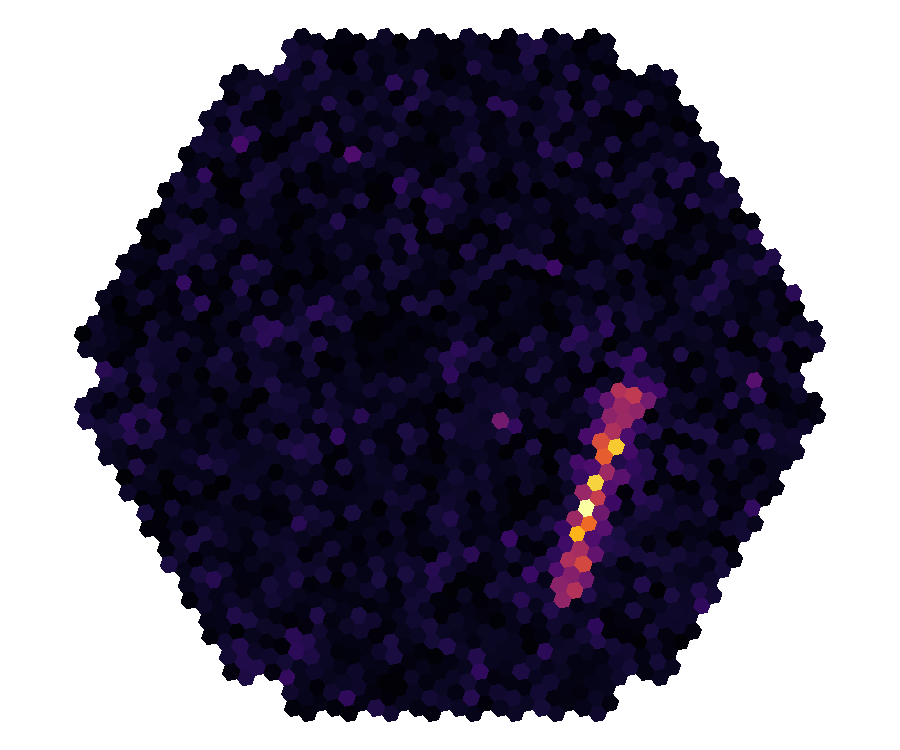
\includegraphics[height=2.8cm]{graphics/mst_camera_frame.pdf}};
        }] (CAMERAFRAME) at (-0.5,2) {};

      % \draw [white, ->, >=latex, every node/.style={font=\sffamily\small}] ;
      \path[white, every node/.style={font=\sffamily\small}, ->, >=latex] (3.2,2.6) edge[bend right] (CAMERAFRAME);


      % \node [white, rotate=45, opacity=0.7] at (4,4) {\Huge WORK IN PROGRESS};

      \end{tikzpicture}
\end{document}
